% #############################################################################
% This is Chapter 2
% !TEX root = ../main.tex
% #############################################################################
% Change the Name of the Chapter i the following line
\fancychapter{Related Work}
\cleardoublepage
% The following line allows to ref this chapter
\label{chap:relatedwork}

In this section, we start by describing and analyzing the most popular music streaming services and the value they add to its millions of users. Then, we study how traditional terrestrial radio has kept up the pace and, despite its competition in the digital era, remained an important and prominent medium.

Finally, we outline the concept of interactive radio by presenting several important projects that apply and augment this concept, followed by a discussion regarding the most attractive and less compelling features of these three audio listening experiences.

% #############################################################################
\section{Music Streaming Services}
\label{subchap:mss}
Music streaming services allow user access to millions of musical content from any web-connected computer, legally and free or with a low charge ~\cite{Swanson2013}. This kind of service marked an important cultural shift from old to new media ~\cite{Glantz2016}. But what attracts listeners to these services?

Various studies have explored the factors that determine consumers’ decisions about adopting digital music streaming services. Vlachos et. al ~\cite{Vlachos2003} identified content and convenience attributes as key indicators of consumers' willingness to use music streaming services. According to Weijters et. al ~\cite{Weijters2014}, there are eight main factors that drive users to adopt these services: audio quality, business model, legality, ethicality, video capability, search/suggest features, connection to social media, and delivery mode (download vs. streaming). Furthermore, Stark et. al ~\cite{Stark2013} have concluded that listeners rely on streaming services primarily for recreation and relaxation and that their listening sessions can happen over an entire day. Glantz et. al ~\cite{Glantz2016} has studied how streaming music services create and embrace opportunities to fit themselves into the lives of music fans while comparing them with terrestrial radio, while Swanson ~\cite{Swanson2013} has studied what users expect from listening to streaming services as an interactive medium, and what are the gratifications sought when tuning into them, also in comparison to terrestrial radio. Finally, Datta et. al ~\cite{Datta2018} have studied how the adoption of music streaming services affects listening behavior of users. 

Spotify, Apple Music, and Pandora Radio are the most used streaming services in the world~\footnote{As of February 2020, according to  \href{http://www.statista.com/chart/20826/music-streaming-services-with-most-subscribers-global-fipp/}{Statista}.}. To understand what are the best functionalities of each platform, we have conducted a study where we analyzed these three platforms with their top-tier plan, for an entire week as our main music listening source. In the ambit of our work, we have focused our analysis on two main aspects of each service: radio and sociability. We have reported our opinions, desires, and aspirations while using each service, so we could analyze their main strong features. The following subsections summarize our conclusions and combine them with researched information about each service.

\subsection{Spotify}
The Sweden-born Spotify\footnote{\href{https://www.spotify.com/}{Spotify website}.} is the most used streaming service in the world. In this service, music can be browsed using a search tool by track name, artist, or album. Users have the option of registering for a free account, supported by visual and radio-style advertising, or for one of two paid subscription models, which are ad-free and offer a range of additional features, such as higher bit rate streams and offline access to music. ~\cite{Swanson2013}

Nowadays, the platform incorporates highly advanced technologies, such as artificial intelligence and machine learning algorithms, in order to be a powerful tool for discovering new music according to the users' tastes. Furthermore, Spotify also provides its users many types of content, such as podcasts and even videos submitted by artists.

One of the main features available on this platform is the 'Radio' section. When using it, Spotify will suggest the user a number of playlists (called 'radio stations') based on their listening habits (favorite genres, artists, albums, or songs). A user is able to create a radio station based on a choice of a song, album, artist, or playlist, and the service will generate a 'radio station' with songs that are similar to the ones selected. As we'll discuss later, many music streaming services, including Spotify, want customers to know that they are similar to, but ultimately different from, or better than, traditional terrestrial radio \cite{Glantz2016}.

\begin{figure}[h]
\centering
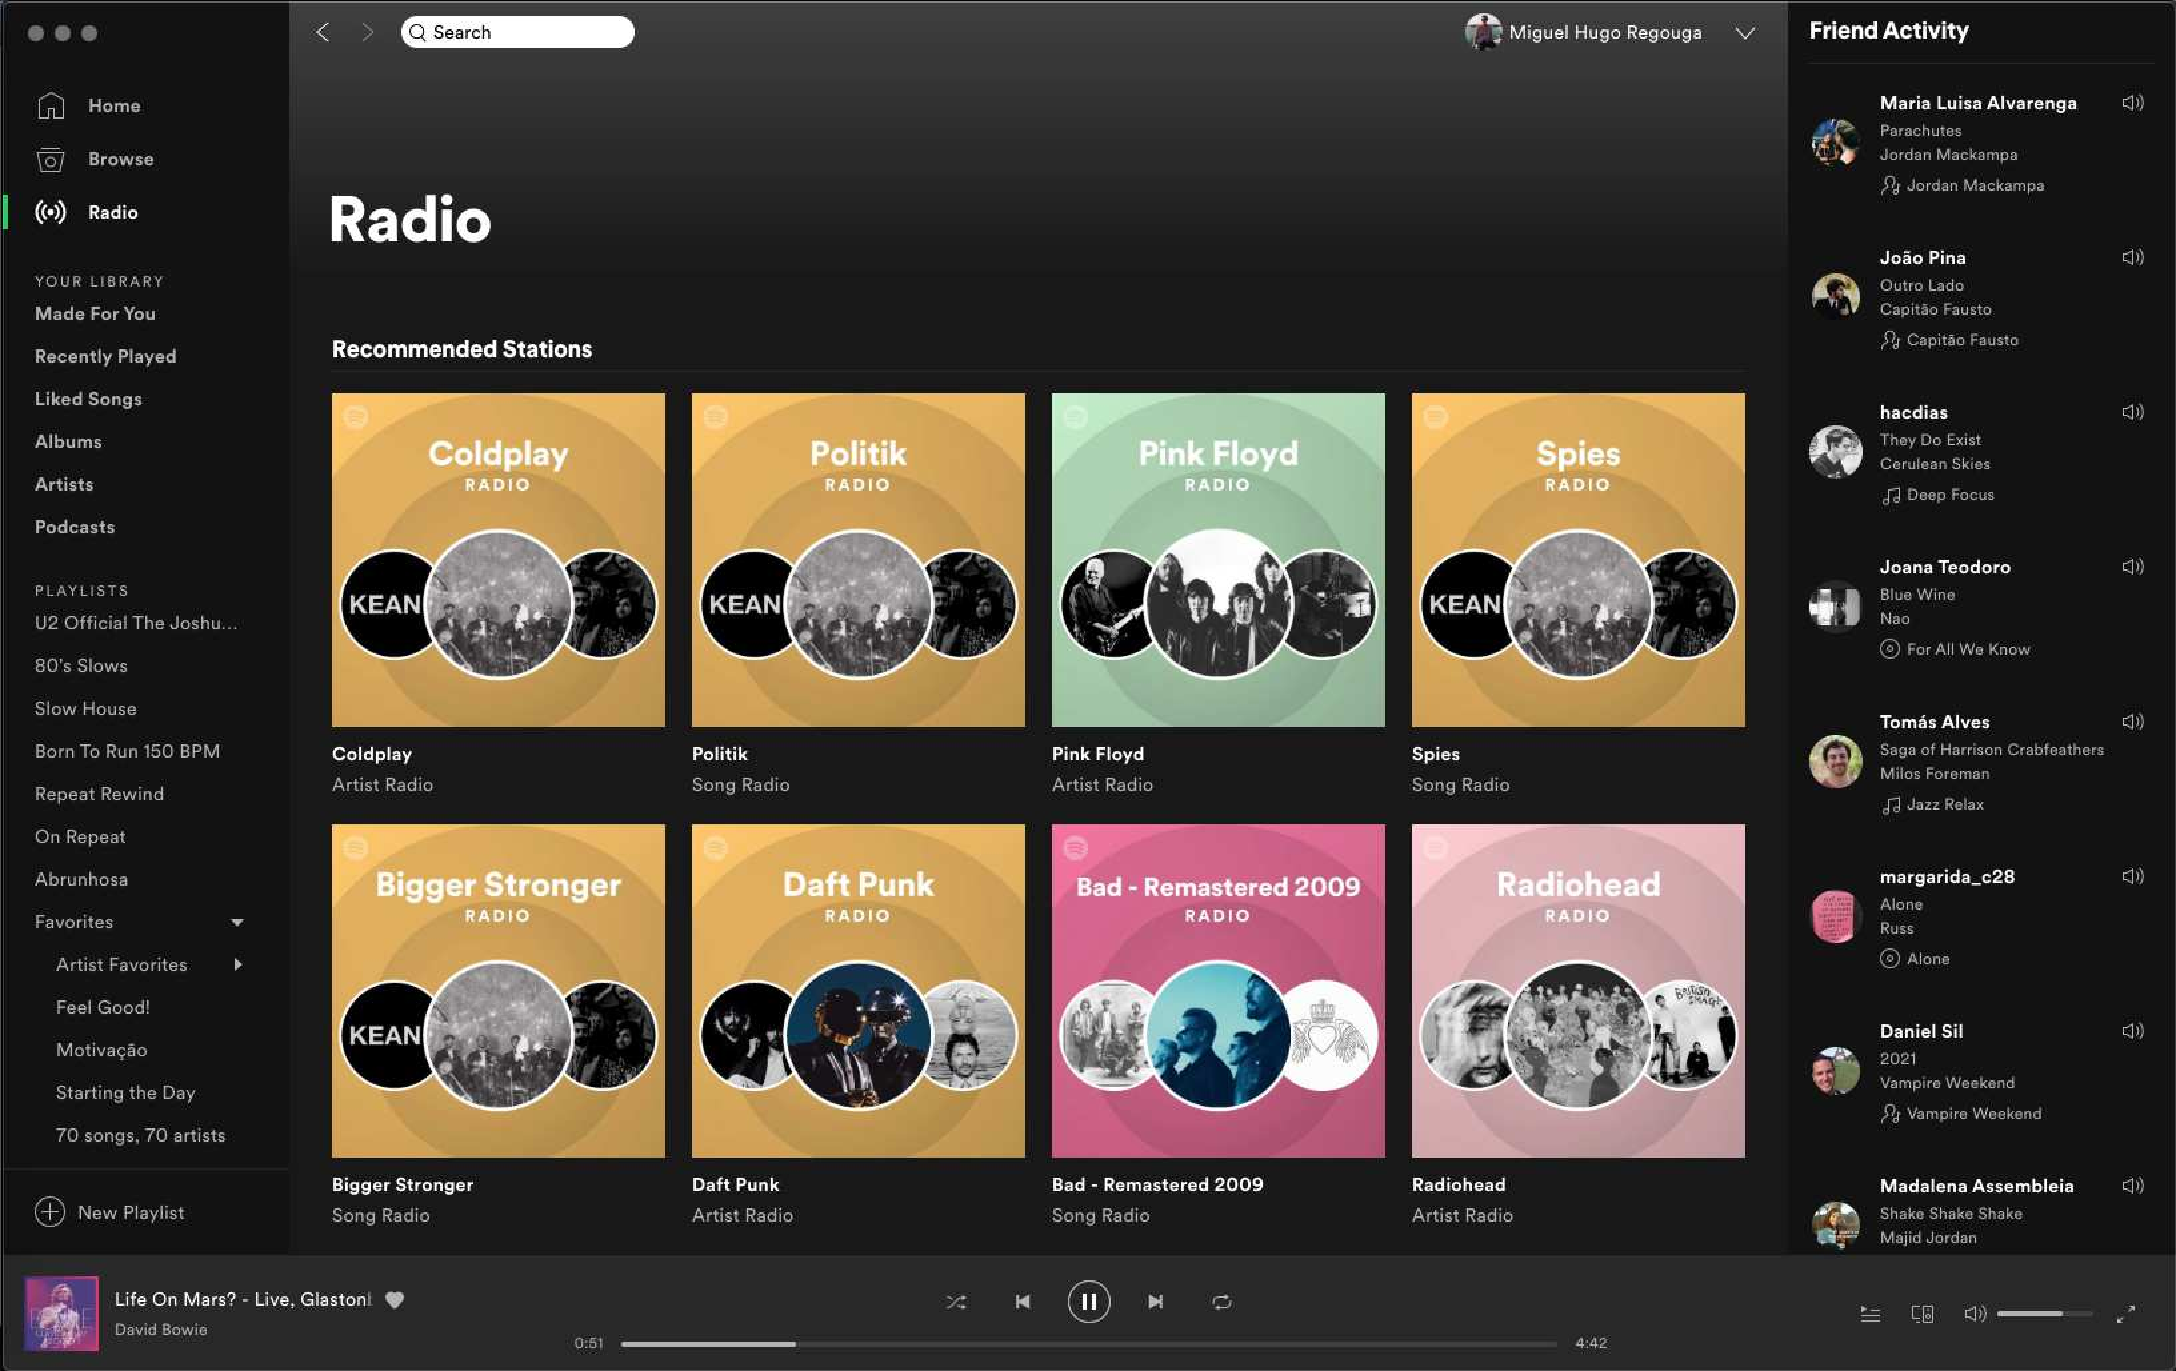
\includegraphics[width=0.8\textwidth]{./Images/spotify.png}
\caption{Spotify 'Radio' discovery features on its desktop application}
\label{fig:test_env}
\end{figure}

Ultimately, the most relevant aspect in the context of our research was Spotify's sociability features. Users can choose from a wide range of playlists created by the Spotify community with hand-picked songs, and not by an algorithm. Furthermore, it is possible to see what friends and family are currently listening to. As Wang et. al ~\cite{Wang2014} described, users of these platforms can be driven by a sense of online community and may be willing to have more interaction with others, and this emphasis on sociability from the inception of the platform might be one of the reasons why it is so popular.

In the context of this project, we consider Spotify as a solid starting point for further analysis and study. It is, according to our criteria, the most solid and robust streaming service available, but has its flaws. As Gunawardena et. al ~\cite{Gunawardena1997} mentions, users can perceive a feeling of warmth and human contact by means of social presence, and although they exist, we find the social features of Spotify quite limited and not enough to provide users a well founded human connection. We'll explore this matter in section ~\ref{sec:methodology}, when we discuss the conducted user research.

\subsection{Apple Music}

In spite of Spotify being currently the most used music streaming service in the world, Apple Music is growing at a fast pace, as it is now the most used streaming service in the United States.\footnote{As of September 2019, reported by \href{https://www.statista.com/statistics/798125/most-popular-us-music-streaming-services-ranked-by-audience/}{Statista}.} The service was born in 2015 after the company Beats was bought by Apple.

When this service was released to the public, its main selling point was that it was bringing a strong human element to these on-demand services, arguing that "algorithms can't do it alone – you need a human touch"~\footnote{\href{https://www.theguardian.com/technology/2015/jun/09/apple-music-interview-jimmy-iovine-eddy-cue}{Apple Music interview: 'Algorithms can't do it alone – you need a human touch' — The Guardian, 2015}}. Thus, the core features of the service were curated playlists, hand-picked by music experts, and recommendations tailored to the users' music preference, not resorting to algorithms (as Spotify does)~\footnote{\href{https://www.theguardian.com/technology/2015/jun/08/apple-music-streaming-service-wwdc-spotify}{Apple unveils streaming service Apple Music and 24-hour radio stations — The Guardian, 2015}}.

Apple Music was also focused to emphasize on traditional terrestrial radio. Along with the introduction of this service, Apple announced they would be launching the Beats 1 radio station (now renamed to Apple Music 1), which broadcasts live to over 100 countries 24 hours a day, and would feature 'real' radio hosts, such as DJ Zane Lowe~\footnote{\href{https://www.theguardian.com/music/2015/feb/16/zane-lowe-apple-bbc-london-radio1-la}{Zane Lowe on Apple, the BBC and why he’ll miss London — The Guardian, 2015}}. In 2020, Apple expanded this section of the service by adding three more 'real' radio stations that offer not only daily curated playlists of music, but also artist interviews, global exclusives and premieres, and other breaking music news. The idea behind these streaming radio stations is to cater to people who, sometimes, just want to turn on music without having to think about what they want to hear or dig around for a favorite playlist. That was the original promise of terrestrial radio, and Apple believes the formula can still work on modern-day streaming services, as well~\footnote{\href{https://www.theguardian.com/music/2015/feb/16/zane-lowe-apple-bbc-london-radio1-la}{Apple launches Apple Music Radio with a rebranded Beats 1, plus two more stations — TechCrunch, 2020}}.

\begin{figure}[h]
\centering
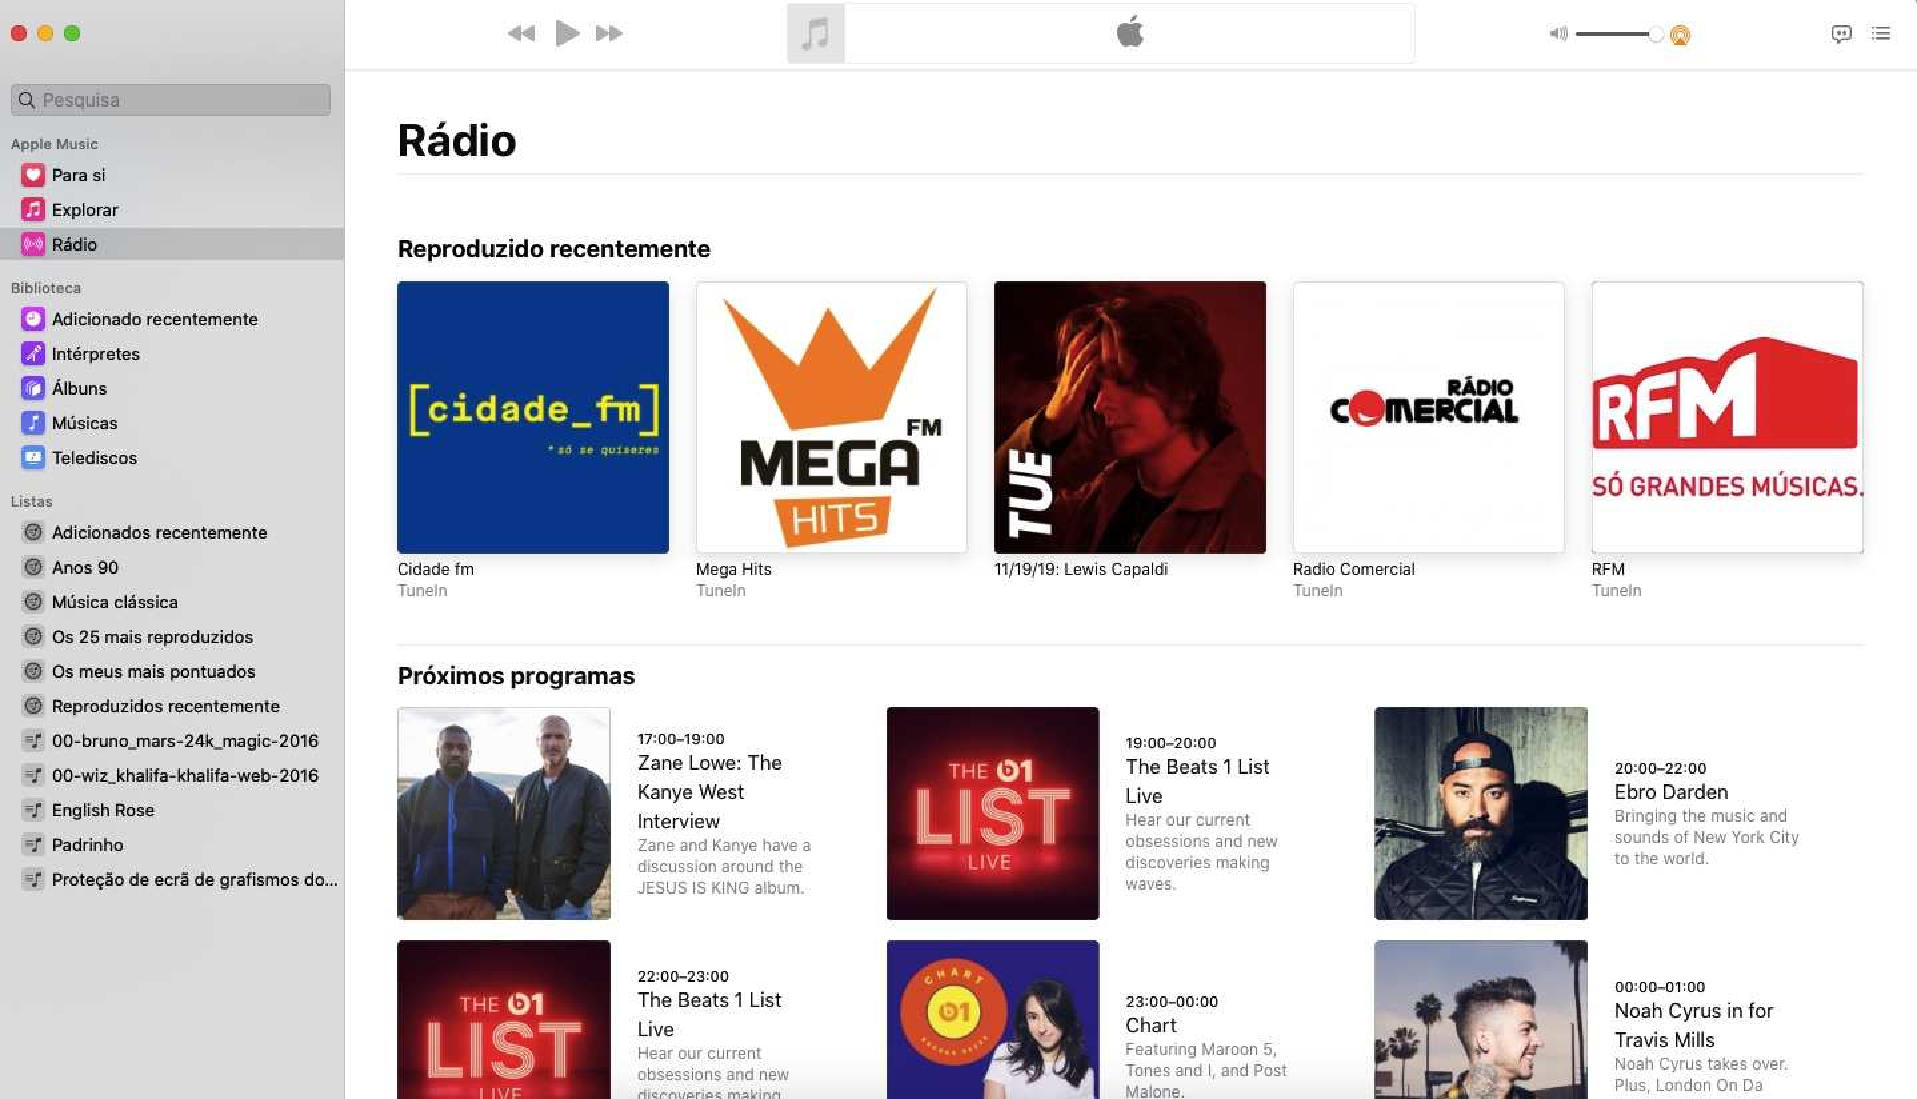
\includegraphics[width=0.8\textwidth]{./Images/applemusic.png}
\caption{Local radio stations and discovery features on the Apple Music 'Radio' tab}
\label{fig:test_env}
\end{figure}

Building on that premise, Apple has also added to the service the ability to search for 'real' radio stations from around the world, allowing users to dial in local broadcast stations by call sign, name, or frequency ~\footnote{\href{https://www.broadbandtvnews.com/2019/09/25/tunein-brings-over-100000-radio-stations-to-apple-music/}{TuneIn brings over 100,000 radio stations to Apple Music — Broadband TV News, 2019}}. Furthermore, the "Radio" tab also incorporates the before-mentioned Apple Music 1 station, as well as other radio stations that play genre-specific or artist-related music, depending on the user's preference. Unlike traditional radio services, the radio feature in Apple Music allows users to skip songs, view previously played tracks on the station, as well as to know what songs are playing next.

In terms of sociability, Apple Music is lacking in features, specially in comparison with Spotify. Although its original release included a 'Connect' screen aimed at creating a social experience between listeners and artists, such feature was later removed due to its low usage~\footnote{\href{https://www.theverge.com/2018/12/13/18139837/apple-music-connect-social-network-feature-discontinued}{Apple is shutting down Apple Music’s rarely-used Connect feature — The Verge, 2018}}. Nevertheless, until 2018, a truly social experience between the platform's users never existed. The ability for users to share what they're listening with their friends was later added~\footnote{\href{https://www.theverge.com/2017/6/5/15727014/apple-music-app-update-social-features-wwdc-2017}{Apple Music will let you share what you’re listening to with your friends — The Verge, 2017}}, yet it is not as developed nor integrated in the platform as Spotify's matching features are.

The approach Apple Music takes on traditional terrestrial radio is very interesting in the ambit of this project. The addition of 'real' radio stations to the service and the commitment to add the option to listen to terrestrial radio stations may prove that users still want to indulge on this medium, despite the convenience that on-demand music selection provides them. Later on the study, we'll analyze the possible reasons why this is happening.

\subsection{Pandora Radio}

The Pandora Radio project was born in 2000, and it is considered one of the oldest streaming services available. The platform is widely popular in the United States, which is the only country it operates in.

Pandora takes on a different approach than the one from Spotify and Apple Music. While both these services were built on an on-demand philosophy, allowing the user to select their desired musical content to play, Pandora wasn't. Pandora enables the creation of 'personal radio stations', in which the user is prompted to choose a song, artist, or album, and a radio station is generated based on that choice (much like the Spotify's own 'radio' feature). ~\cite{Meneses2012} In short, listeners can tune into established genre stations, other users' stations, or create their own stations based on their musical interests. It functions in a similar way to a traditional radio station except that users select a song or artist they want to hear and a station is generated based upon such selection. ~\cite{Swanson2013}

\begin{figure}[h]
\centering
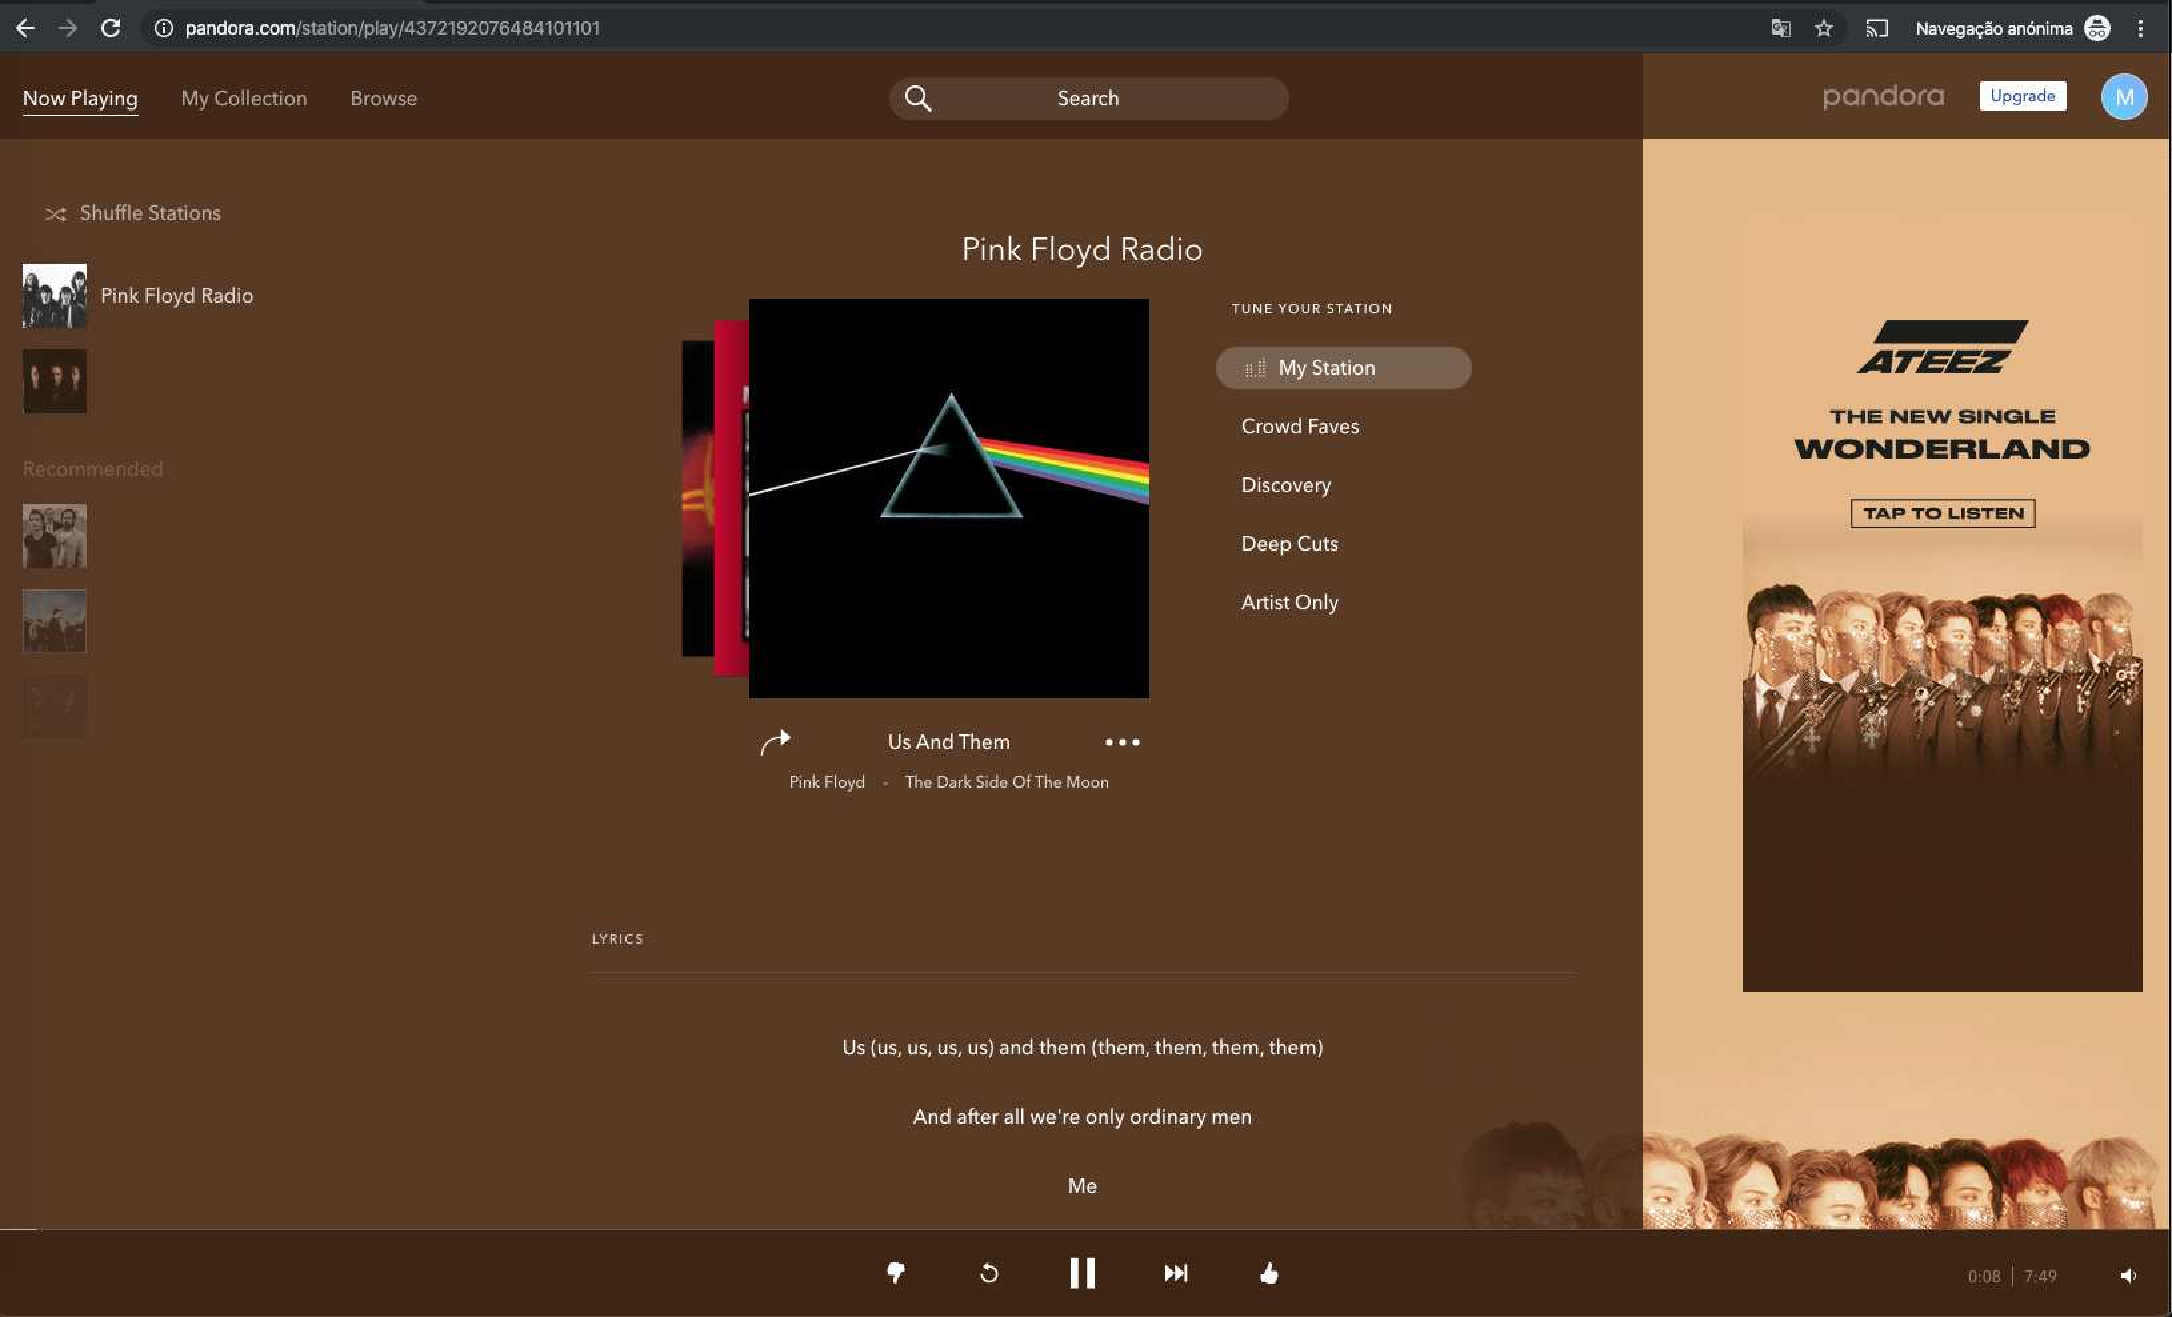
\includegraphics[width=0.8\textwidth]{./Images/pandora.png}
\caption{Pandora Radio web interface}
\label{fig:test_env}
\end{figure}

While listening, users can rate positively or negatively the songs that are being played, and such feedback is taken into account in the subsequent selection of other songs to play, tuning in each station to the users' taste. Furthermore, users may even tailor their station to specific tendencies, such as 'Discovery', 'Crowd Faves', or 'Deep Cuts'.

When talking sociability, Pandora offers the same basic social functionalities as Apple Music — it is possible to follow users, see what they are listening to, and share stations with the community, but the platform isn't as community-centered as Spotify is.

One of the reasons Pandora may be so widely used is the fact that users don't want to choose what they want to listen to all the time. As Meneses mentioned ~\cite{Meneses2012}, having millions of songs available is perfect when users want to listen to the music they are already familiar with, but most users don't want to listen to the same music constantly - hence the creation of discovery features on Spotify and Apple Music. On the other hand, if traditional radio is the main information source on new music, that happens because users want to uncover new material from artists or genres.

%\subsection{Analysis}
%%Tabela comparativa dos music streaming services
%
%Audio streaming services are used daily by millions worldwide, enabling on-demand listening and the discovery of songs, artists and podcasts that closely align with the listener’s preferences. Around the world, there are more than 30 of these platforms available, but the most used ones are Spotify, Apple Music, and Pandora Radio.
%
%Each one of these services offers a unique and enticing set of features to their users. To facilitate the comparison between each service's functionalities, Table ~\ref{tab:mssfeatures} was created, with the lines showcasing the before-mentioned three most popular music streaming services, and the columns showing some cross-cut features of these services, which are:
%
%\begin{itemize}
%\item (a) On-demand music selection
%\item (b) ‘Real’ radio stations
%\item (c) Song discovery features
%\item (d) Shared playlists
%\item (e) Social feeds
%\item (f) Group listening
%\end{itemize}
%
%These functionalities were selected as we consider them to be the most relevant and prominent in the ambit of our case study. 
%
%By analyzing the table, we can conclude that, at a first glance, Spotify is the most robust service of the three, while Pandora Radio is the most limited one. All three services have a very limited set of social features — most importantly, they all lack a true social feed functionality. Although Spotify does offer a 'listening activity' feature, where users can follow and see what other users are listening to, this feature is very limited as it is only available on the desktop counterpart of the service
%
%\begin{table}[]
%\centering
%\resizebox{0.8\textwidth}{!}{%
%\begin{tabular}{|l|c|c|c|c|c|c|}
%\hline
%              & (a)                         & (b)                         & (c)                                                & (d)                         & (e)                        & (f)                         \\ \hline
%Spotify       & \cellcolor[HTML]{34FF34}Yes & \cellcolor[HTML]{FFCCC9}No  & \cellcolor[HTML]{34FF34}{\color[HTML]{333333} Yes} & \cellcolor[HTML]{34FF34}Yes & \cellcolor[HTML]{FFCCC9}No & \cellcolor[HTML]{34FF34}Yes \\ \hline
%Apple Music   & \cellcolor[HTML]{34FF34}Yes & \cellcolor[HTML]{34FF34}Yes & \cellcolor[HTML]{34FF34}Yes                        & \cellcolor[HTML]{FFCCC9}No  & \cellcolor[HTML]{FFCCC9}No & \cellcolor[HTML]{FFCCC9}No  \\ \hline
%Pandora Radio & \cellcolor[HTML]{FFCCC9}No  & \cellcolor[HTML]{FFCCC9}No  & \cellcolor[HTML]{34FF34}Yes                        & \cellcolor[HTML]{FFCCC9}No  & \cellcolor[HTML]{FFCCC9}No & \cellcolor[HTML]{FFCCC9}No  \\ \hline
%\end{tabular}%
%}
%\caption{Summary of the analyzed music streaming services' features}
%\label{tab:mssfeatures}
%\end{table}



\section{Traditional Terrestrial Radio}
\label{chap:ttr}
Radio is the first mass medium that enables the instant dissemination of information from one to many, and it is often described as a "local" and "personable" medium to its audience ~\cite{Ren2004}. It is largely a one-way communication system that allows individual listeners to passively consume radio content provided by radio broadcasters without any interaction or participation ~\cite{Gazi2011}. From its inception, traditional terrestrial radio has been challenged by several innovative technologies, each drawing listeners and forcing radio to update its programming to remain a competitive media option ~\cite{Albarran2007}. 

\begin{figure}
 \centering
	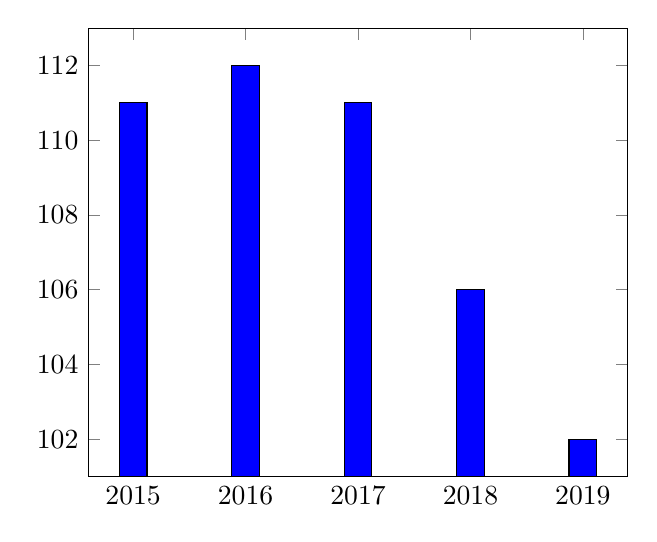
\begin{tikzpicture}
\begin{axis}[
    symbolic x coords={2015,2016,2017,2018,2019},
    xtick=data]
    \addplot[ybar,fill=blue] coordinates {
        (2015,111)
        (2016,112)
        (2017,111)
        (2018,106)
        (2019,102)
    };
\end{axis}
\end{tikzpicture}
\caption{Average daily time spent listening to the radio per adult in the United States (in minutes) —  Statista}
\label{fig:test_env}
\end{figure}


Although music plays a vital role in radio diffusion, traditional terrestrial radio also provides its listeners with useful information, such as news, weather, and traffic reports. A study conducted by Albarran et. al ~\cite{Albarran2007} has shown that, when taking all other audible mediums available into account (including music streaming services), traditional radio is still ranked as the first go-to solution when a user wants to access news and other types of information. 


Waits et. al ~\cite{Waits2007} states that traditional radio still features one of the things that on-demand streaming services may arguably be taking away from its users — a human connection, stating that the users' relationship to this medium is determined by a certain expectation that it will be authentic, sociable, and display intentionally and sincerity. Priestman et. al ~\cite{Priestman2005} argues that the same cannot be said about music streaming services, naming these platforms as 'automated music channels' or 'automated web jukeboxes', due to the absence of the sociable component in conjunction with the emphasis on the listener's music selection. The researchers' approach on traditional radio can be defined as a 'human communication', where one senses that the voice of an announcer creating the threads between various other broadcast elements becomes a key point. 

A different study, conducted by Glantz et. al ~\cite{Glantz2016}, states that, as advanced as music streaming platforms can be, they still anchor themselves in traditional radio. Many of these services market themselves as a "personalized radio", "your radio station", or as far as "radio reimagined". They want their users to believe that they are similar to, but ultimately different from, or better than, traditional terrestrial radio. In contrast, Priestman et. al ~\cite{Priestman2005} describe streaming services as a contradictory phenomenon to define in radio terms, since "it is quite clearly an extension of music format radio but, in doing away with any form of presenter or news or indeed any kind of radio studio at all, it removes the essential element of broadcast communication: one human person talking directly to another or sharing with them some form of entertainment."

In a study conducted in 2008 by Ala-Fossi et. al ~\cite{Ala-Fossi2008}. a group of users predicted that that the numbers of FM radio stations and their listeners would be decreasing by 2015, due to the impact of the emerging internet services, such as music streaming platforms. Yet, in defiance of the competition, traditional radio remains the biggest mass-reach medium in the United States, with more than 90\% of consumers listening on a weekly basis ~\footnote{\href{https://qz.com/195349/the-remarkable-resilience-of-old-fashioned-radio-in-the-us/}{The remarkable resilience of old-fashioned radio in the US — Quartz, 2014}}. The main thesis on why this is happening has to do with the conjunction of two concepts: passive listening, to which traditional terrestrial radio is built upon on; and tyranny of choice. ~\footnote{\href{https://qz.com/1094963/radio-survived-the-tape-cd-and-ipod-in-the-age-of-spotify-its-more-popular-than-ever/}{Radio survived the tape, CD, and iPod. In the age of Spotify, it’s more popular than ever. — Quartz, 2017}} According to Miller, “the availability of so much music has led to what some academics and analysts call the tyranny of choice". Users of music streaming platforms are often hit by this tyranny of choice, where the amount of selection available makes them unable to decide what to listen to, tuning to a 'traditional' radio station where a radio host interacts passively with its listeners. ~\cite{Pedersen2014}.

In short, terrestrial radio still remains with a strong adoption, in spite of the rise of on-demand services. The disclosure of information, the passive audio listening experience, the sense of community, or the human connection that terrestrial radio stations provide may be some of the reasons why users still indulge heavily on this traditional medium. Nevertheless, music streaming services are still rising in popularity, which proves that the convenience of on-demand listening is evident among its users. The concept of interactive radio, which will be discussed in the following section, may provide a hint at a solution that aims to pick on the passive experience of traditional radio and merge it with the on-demand music selection that streaming services provide.

\section{Interactive Radio}

\subsection{Calm Computing}

In 1991, Weiser and Brown suggested that “if computers are everywhere they better stay out of the way, and that means designing them so that the people being shared by the computers remain serene and in control.” ~\cite{Weiser1997} Weiser and Brown’s vision was not realised, as nowadays computers are everywhere, but they do not stay out of our way. Mobile computing is predominantly stop-and-interact and the web demands our constant engagement. Yet, there might be a platform available for a pervasive service that could advance Weiser and Brown’s vision of calm computing: the format of radio.

Audio is an example of content which we can selectively attend to. Many times users listen to music while they do something else: work, run, drive, etc. Vazquez-Alvarez et. al ~\cite{Vazquez-Alvarez2011} showed that, when designing audio interfaces, there was a significant difference between the user experience of selective attention (where audio was in the background and not requiring the full attention of the user) and divided attention (when two audio streams where competing for the user’s attention). This ability for audio to shift between the center of our attention and its periphery fulfills a key element of Weiser and Brown’s vision of calm computing.~\cite{Weiser1997} Calm computing argues that systems should remain in the periphery of our attention until we require their services, at which point they would move to the center of our attention for direct interaction.

Radio is so common as a passive medium that it requires a conceptual leap to regard radio as a possible platform for eyes-free interaction. Yet, similar to interactive television, the concept of interactive radio is not a recent one. Although radio is considered to be a one-way communication channel from station to listener, many radio hosts try to mitigate this by asking listeners to interact with them — either through more analog types of communication, such as phone calls, or using modern platforms such as WhatsApp, enabling the listener to interact more easily with radio stations, potentially augmenting the overall experience of the listener. ~\cite{Claes2018, Ren2004} Yet, in the prime age of social interaction, many researchers have studied how this concept may be taken even further.

\subsection{Nomadic Radio}

One of the first approaches to this concept was presented by Sawhney et. al ~\cite{Sawhney1999} in 1999. The researchers developed a system called \textit{Nomadic Radio} in which scaleable auditory techniques and contextual notification modules for providing timely information were applied, while minimizing interruptions.

\begin{figure}[h]
\centering
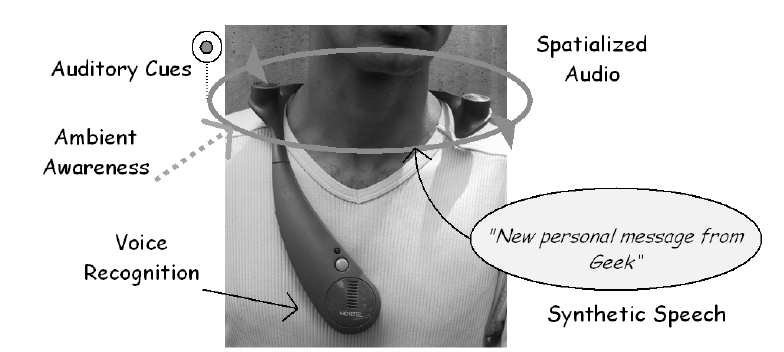
\includegraphics[width=0.8\textwidth]{./Images/nomadicradio.png}
\caption{Description of the Nomadic Radio system with the SoundBeam Neckset audio device}
\label{fig:test_env}
\end{figure}

Nomadic Radio is a wearable computing platform that provided a unified audio-only interface to remote services and messages such as email, voice mail, hourly news broadcasts, and personal calendar events. These messages are automatically downloaded to the device throughout the day and users can browse through them using voice commands and tactile input. This first attempt was, however, targeted at mobile workers rather than at the general audio media consumer.

\subsection{AudioFeeds}

Dingler et. al ~\cite{Dingler2010} built on the \textit{Nomadic Radio} concept and took a more user-centered approach by proposing a mobile auditory display application, called \textit{AudioFeeds}, that allowed users to maintain an overview of activities in different social feeds. The application runs on a mobile device and enables users to get an overview of their social networks and spot peaks in activity by sonifying social feeds and creating a spatialised soundscape around the user’s head. By using this solution, users could stay informed about current issues and spot ‘hot topics’ while on the go. 

\begin{figure}[h]
\centering
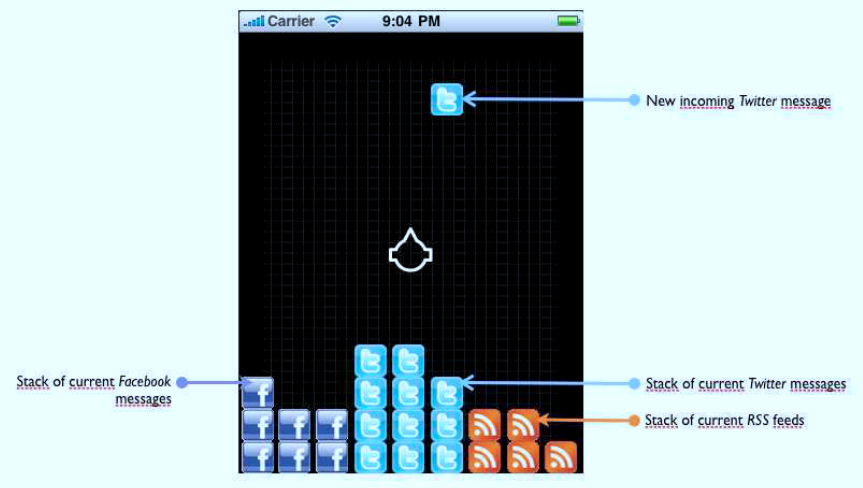
\includegraphics[width=0.8\textwidth]{./Images/audiofeeds.png}
\caption{AudioFeeds GUI, where incoming messages are represented by icons that are dropped from the top}
\label{fig:test_env}
\end{figure}

\textit{AudioFeeds} adapted the idea of adaptive notifications that \textit{Nomadic Radio} introduced and applied it to social feeds and their activity levels. The system enabled users to easily make out interesting social feed activities while maintaining an overview even in complex streams of information, thus fulfilling Weiser’s vision of calm computing~\cite{Weiser1997} and forming a close approximation of a truly interactive radio platform.


\subsection{Radialize}

More recently, Pereira et. al ~\cite{Pereira2013} created a platform for listening to music and radio programs through the Web, allowing the discovery of the content being played by radio stations on the Web, either by managing explicit information made available by those stations or by means of our technology for automatic recognition of audio content in a stream. Users can search, receive recommendations, and provide feedback on artists and songs being played in traditional radio stations, either explicitly or implicitly, in order to compose an individual profile.

\textit{Radialize} utilizes every user interaction as a data source, as well as the similarity abstraction extracted out of the radios’ musical programs, making use of the wisdom of crowds implicitly present in the radio programs. The system was one of the first user-available platforms that introduced a novel social listening experience based on the radio format, aiming to "be responsible for the transition of radio stations as a kind of mass media to a kind of social network".~\cite{Pereira2013}


\begin{figure}[h]
\centering
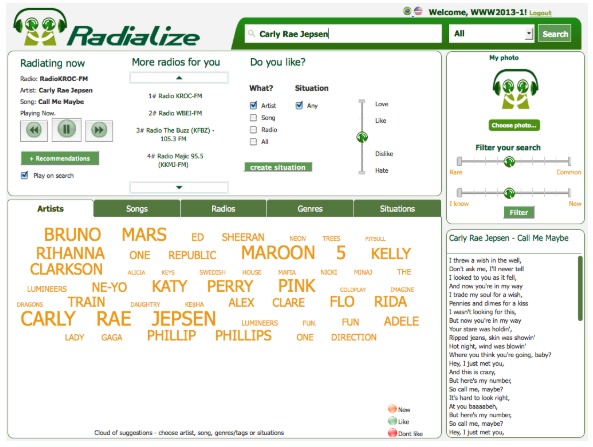
\includegraphics[width=0.8\textwidth]{./Images/radialize.png}
\caption{Screenshot of the Radialize system}
\label{fig:test_env}
\end{figure}

\subsection{MyMyRadio}

Finally, and most importantly, the CereProc team created a platform which takes updates from a user's Facebook or Twitter accounts, and RSS feeds, and synthesizes them using CereProc's own text to speech technology, slotting these spoken updates into a playlist of your own music periodically. ~\footnote{\href{https://www.cereproc.com/en/mymyradio}{MyMyRadio (https://www.cereproc.com/en/mymyradio)}} Aylett et. al~\cite{Aylett2015} have presented a case study on this platform, in which they highlight the potential and challenges of an interactive radio approach, which are of interest to the development of this project.

The MyMyRadio project was developed as a 'cure' to the constant engagement demanded by social networks, enabling content to be delivered in the background while users listened to music and carried out other activities. When a news or a social media was of interest to the user, the user could embrace a more direct and interactive approach with said content, allowing from an active listening experience. If a social, or news headline was of interest, the user would attend to it more closely and could interact directly with the content, moving from a passive or push-down consumption of content to an active or pull-down consumption.

This is in contrast with systems which use audio as notification of content, such as the previously discussed \textit{Nomadic Radio} and \textit{AudioFeeds}, where an audio notification interrupts the current activity. Instead, MyMyRadio inserts content naturally between music tracks to allow continued attention in the periphery. Furthermore, an audio notification system typically does not render the actual information, whereas MyMyRadio uses speech synthesis to render the headline so that only content which is of interest to users is brought to their attention. According to the testing results, the concept of this platform was well received and considered 'desirable' by its users.

\begin{figure}[h]
\centering
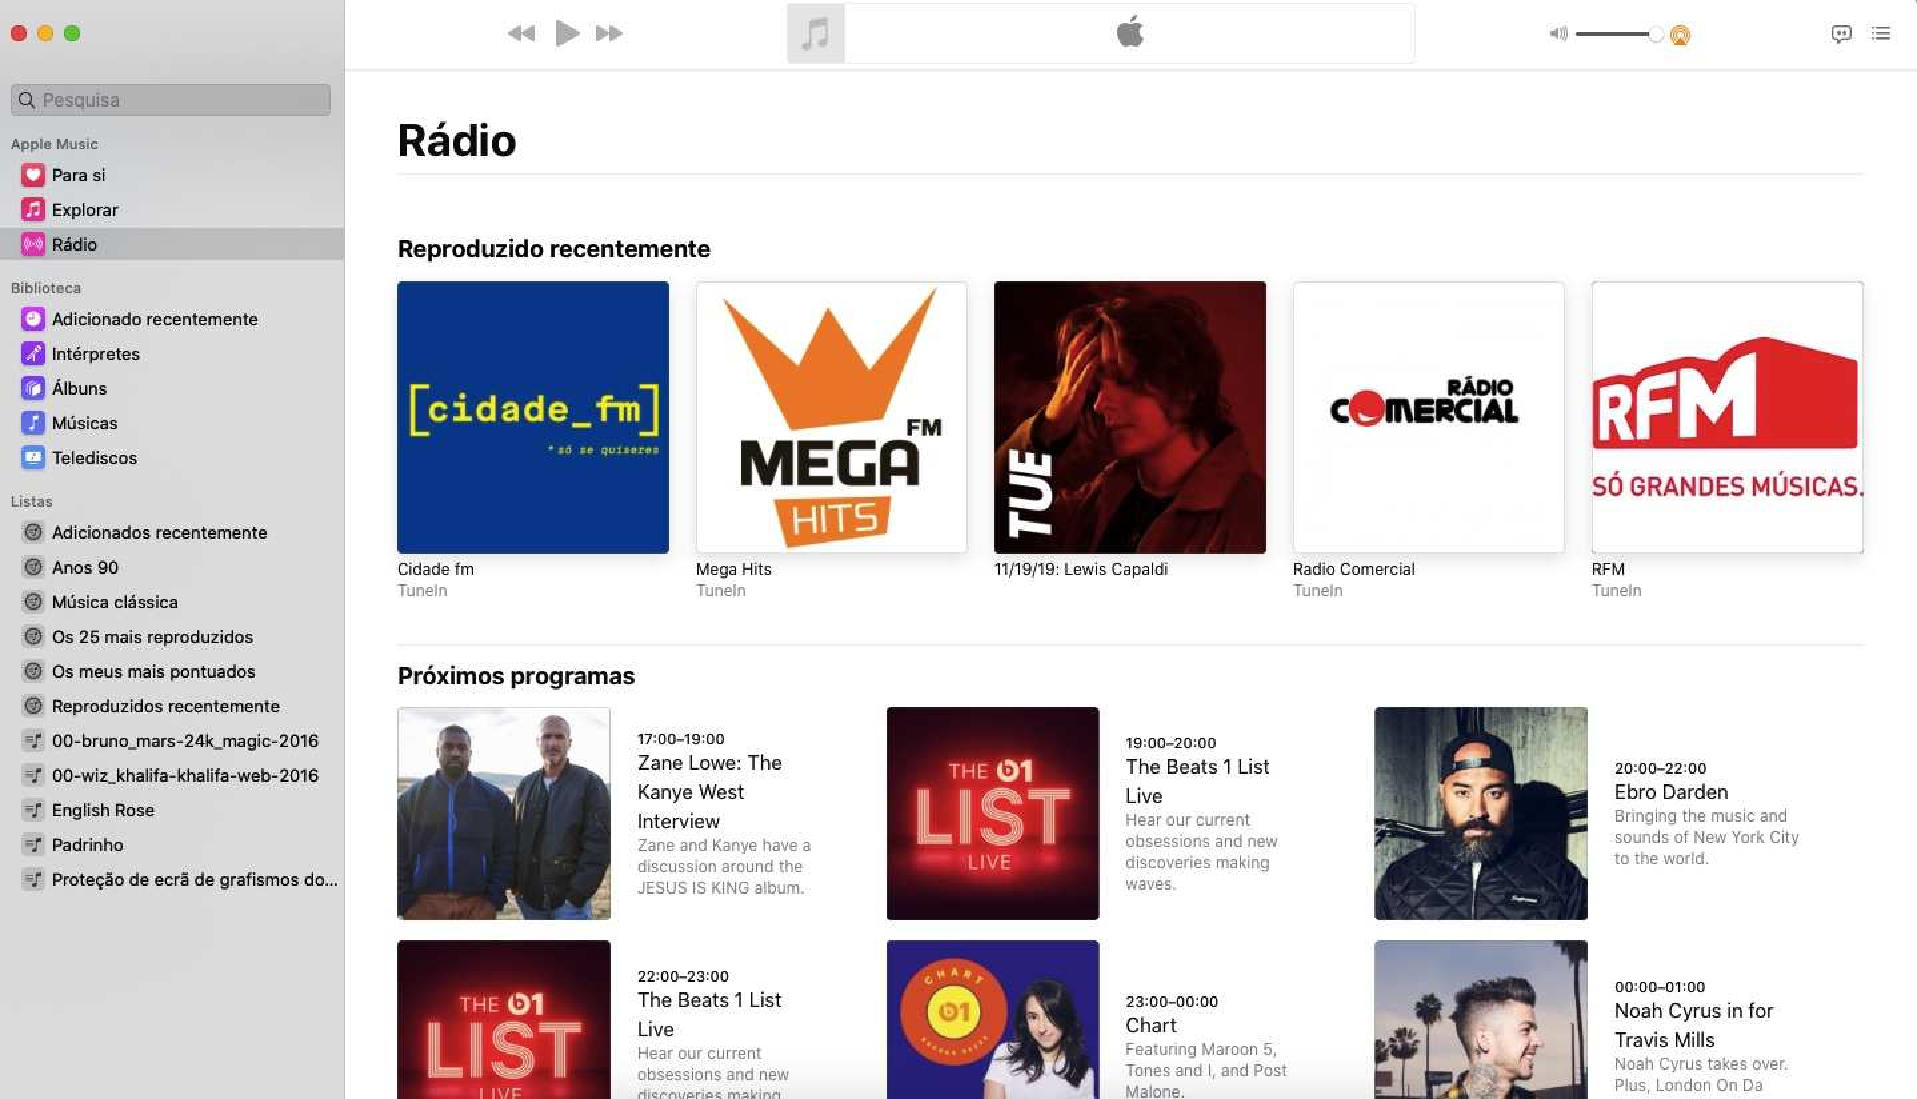
\includegraphics[width=0.8\textwidth]{./Images/applemusic.png}
\caption{MyMyRadio mobile interface}
\label{fig:test_env}
\end{figure}

In the ambit of such case study, the researchers concluded that \textit{'a more developed interactive radio platform could contain localization information and allow a mixture of localized content, speech synthesis and pre-recorded audio, as well as personalized music streams such as Spotify (...) and offer integration with social media and new digital services}.'


\subsection{Analysis}
%Tabela comparativa das interative radio

To facilitate the comparison between the mentioned platforms that implement and augment the interactive radio concept, Table ~\ref{tab:irfeatures} was created, with lines representing a given platform and columns showing some common and relevant features. We selected these features because we consider them to be the most important in the ambit of our case study. The mentioned features are:

\begin{enumerate}[label=(\alph*)]
	\item Audio notifications (interrupts current activity);
	\item News and social feeds (RSS, Facebook, Twitter);
	\item Integration with local (offline) music library;
	\item Integration with music streaming services;
	\item Speech synthesis of information (text-to-speech);
	\item On-site information rendering;
	\item Audio effects (adverts, jingles, background music);
	\item Social network/community features;
	\item Customization and recommendations;
\end{enumerate}


\begin{table}[]
\centering
\resizebox{\textwidth}{!}{%
\begin{tabular}{|l|c|c|c|c|c|c|c|c|c|}
\hline
              & (a)                         & (b)                         & (c)                         & (d)                        & (e)                         & (f)                         & (g)                         & (h)                         & (i)                         \\ \hline
Nomadic Radio & \cellcolor[HTML]{9AFF99}Yes & \cellcolor[HTML]{FFCCC9}No  & \cellcolor[HTML]{FFCCC9}No  & \cellcolor[HTML]{FFCCC9}No & \cellcolor[HTML]{FFCCC9}No  & \cellcolor[HTML]{FFCCC9}No  & \cellcolor[HTML]{FFCCC9}No  & \cellcolor[HTML]{FFCCC9}No  & \cellcolor[HTML]{FFCCC9}No  \\ \hline
AudioFeeds    & \cellcolor[HTML]{9AFF99}Yes & \cellcolor[HTML]{9AFF99}Yes & \cellcolor[HTML]{FFCCC9}No  & \cellcolor[HTML]{FFCCC9}No & \cellcolor[HTML]{FFCCC9}No  & \cellcolor[HTML]{FFCCC9}No  & \cellcolor[HTML]{FFCCC9}No  & \cellcolor[HTML]{FFCCC9}No  & \cellcolor[HTML]{FFCCC9}No  \\ \hline
Radialize     & \cellcolor[HTML]{FFCCC9}No  & \cellcolor[HTML]{FFCCC9}No  & \cellcolor[HTML]{FFCCC9}No & \cellcolor[HTML]{FFCCC9}No & \cellcolor[HTML]{FFCCC9}No  & \cellcolor[HTML]{FFCCC9}No  & \cellcolor[HTML]{FFCCC9}No  & \cellcolor[HTML]{9AFF99}Yes & \cellcolor[HTML]{9AFF99}Yes \\ \hline
MyMyRadio     & \cellcolor[HTML]{FFCCC9}No  & \cellcolor[HTML]{9AFF99}Yes & \cellcolor[HTML]{9AFF99}Yes  & \cellcolor[HTML]{FFCCC9}No & \cellcolor[HTML]{9AFF99}Yes & \cellcolor[HTML]{9AFF99}Yes & \cellcolor[HTML]{9AFF99}Yes & \cellcolor[HTML]{FFCCC9}No & \cellcolor[HTML]{FFCCC9}No  \\ \hline
\end{tabular}%
}
\caption{Summary of the analyzed interactive radio and calm computing platforms}
\label{tab:irfeatures}
\end{table}

The first feature determines if the system uses audio as notification of content, which interrupts the current activity of the listener ~\cite{Dingler2010}. The MyMyRadio system inserts content naturally between music tracks to allow continued attention in the periphery, which can result in an improved experience for the user.

Regarding the more social features, AudioFeeds and MyMyRadio provide integration with various social networks and news aggregation services, but AudioFeeds does not render the information locally as MyMyRadio does. This gives an advantage to the latter platform, which uses speech synthesis to render the headline so that only content which is of interest to users is brought to their attention. ~\cite{Aylett2015} However, although it aggregates displays content from social networks, MyMyRadio doesn't offer a truly social experience between users of the platform, and this is where Radialize has an advantage over the studied platforms.

By analyzing the table, we can observe that MyMyRadio is the most feature-packed platform, closely aligning with the scope of our project. It features a radio-like experience for its users by including audio dynamically created from news and social media sources, integration with the users' local music library, non-speech audio sound effects, and background music. 

Yet, we can observe that none of the studied platforms offer integration with music streaming services, which, as we discussed in section ~\ref{subchap:mss}, are now one of the preferred mediums for consuming audio content. Furthermore, only one platform offers a truly customizable experience tailored to each individual user, while also indulging them in a social-network like atmosphere. Identifying this will be important for defining our window of opportunity and to determine out how we can create a novel listening experience.

In conclusion, the concept of interactive radio can be further augmented, as, at first sight, there is both a user impulse for this to happen, and an opportunity that we can approach and tackle. Based on our research, this may be achieved by merging the strengths of both traditional terrestrial radio and music streaming services into a personal, yet sharable and customizable platform that aims to improve audio media consumers' listening experience. To assure this need, we'll conduct in-depth user research, aiming at understanding if users find such concept enticing.
